\chapter{Theory}

\section{Scientific Computing}



Scientific computing covers a large multi-disciplinary field, typically combining mathematics, computer science and engineering. For this project the most relevant subfield is High-Performance Computing (HPC) which focuses on high performance for short periods \cite{larsen:hpc}, in contrast to High-Throughput Computing (HPT) which focuses on finishing many tasks over a long period \cite{wisc:htcondor}. With the advent of big data, state of the art machine learning has begun intersecting more with the field of HPC.

HPC is typically done on clusters of computers with many CPUs and GPUs, connected through a high-speed communication bus. Workloads not designed for parallelism are not ideal to run on an HPC cluster, as HPC clusters do not perform single core processing particularly better than a server or desktop computer. Software is not perfectly paralellizable and there is always a part that has to be executed sequentially. Using Amdahl's Law \cite{larsen:hpc} in \eqref{eq:amdahl} it is possible to determine the maximum theoretical speedup for a piece of software, based on what percentage that is parallelizable. The variable $S$ means speedup and denotes how many times faster the software can be run as the amount of processors go to infinity. The value $p$ denotes the percentage of the program that is parallelizable and in practice it is impossible for it to be 1.

\begin{equation} \label{eq:amdahl}
    S = \frac{1}{1 - p}
\end{equation}

Figure \ref{fig:amdahl} shows Amdahl's Law for different values of $p$ with a $\log_2$ scaled x-axis. Although a $p$-value of 0.95 can double the speedup compared to a $p-value$ of 0.90, it also requires 4 times as many processors to reach its limit (512 vs. 2048 processors).

\begin{figure}[H]
    \centering
    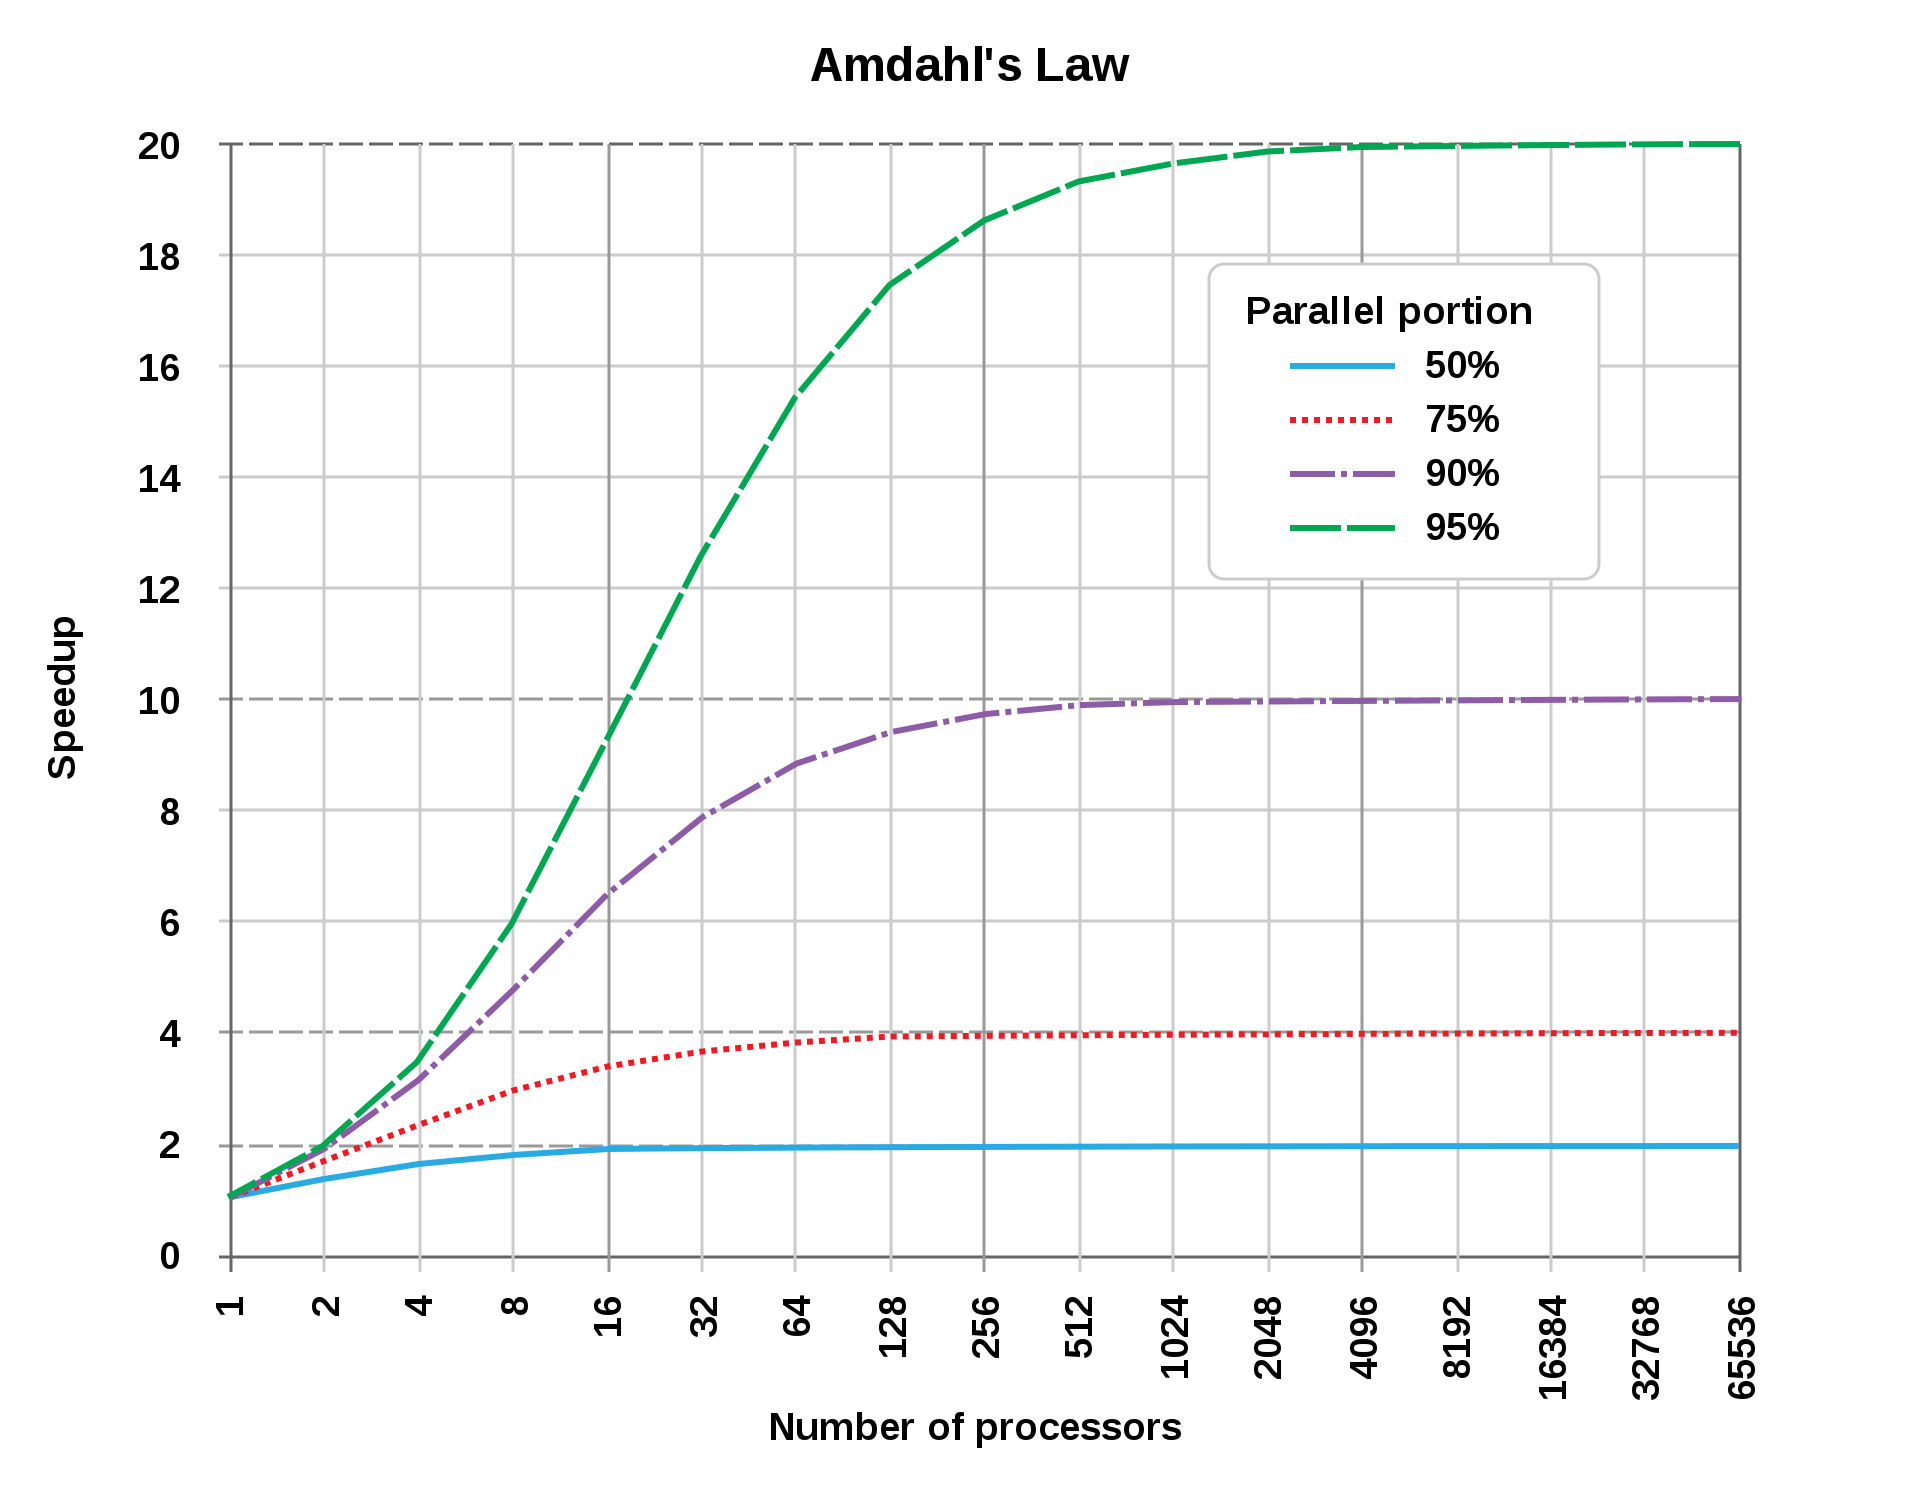
\includegraphics[scale=0.17]{Figures/amdahl.png}
    \caption[]{Amdahl's Law\protect\footnotemark\ with different percentage of parallelism}
    \label{fig:amdahl}
\end{figure} \footnotetext{\url{https://en.wikipedia.org/wiki/Amdahl\%27s\_law\#/media/File:AmdahlsLaw.svg}}

Flynn's Taxonomy in Figure \ref{fig:flynn:taxonomy} shows the different classifications of parallel computer architectures. The two most commonly used computer architectures in HPC are Single Instruction Multiple Data (SIMD) and Multiple Instruction Multiple Data (MIMD). The SIMD aspect in HPC comes from each CPU core and GPU being able to do data parallelism with their vector instructions. GPUs are typically able to compute more things in parallel than CPUs, but GPUs do not compute as many instructions per cycle (IPC) as a CPU. The MIMD aspect in HPC comes from combining multiple devices, which can be either multiple CPU cores, multiple GPUs or both.

\begin{figure}[H]
    \centering
    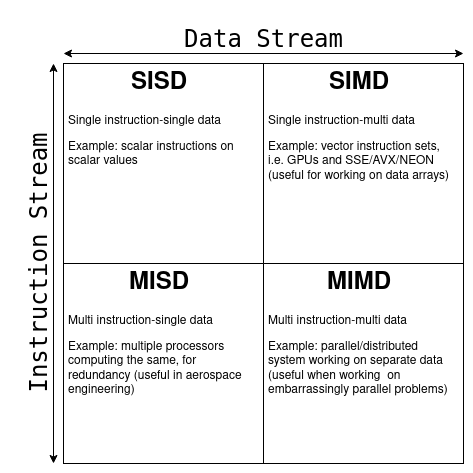
\includegraphics[scale=0.45]{Figures/flynns_taxonomy.png}
    \caption{Flynn's Taxonomy}
    \label{fig:flynn:taxonomy}
\end{figure}

To take advantage of the SIMD and MIMD architectures, libraries can be optimized to utilize multiple CPU cores, GPUs and/or vector instructions. The more popular libraries in HPC are the Basic Linear Algebra Subprograms (BLAS) specification, which specifies a specification for doing vector-vector, matrix-vector and matrix-matrix operations. The BLAS specification does not specify operations for matrix decomposition (i.e. SVD or EVD), but some libraries implementing BLAS also includes support for this.

The benefit of using these pre-existing linear algebra libraries is that a lot of time has already been spent on optimizing performance for their target platform. Intel and NVIDIA both make linear algebra libraries for their hardware platforms. Intel makes the \textit{Math Kernel Library} (MKL) which uses multiple cores and the vector instructions on their CPUs. NVIDIA makes the CUDA based \textit{cuBLAS} and \textit{cuSOLVER} libraries that are designed to run on one or more GPU. Both of these are designed for homogenous hardware, i.e. they cannot utilize both the CPU and GPU. Libraries like MAGMA are heterogeneous libraries, as they use CPU and GPU to compute different parts of a problem. MKL, cuBLAS/cuSOLVER and MAGMA are all MIMD based libraries, but they take advantage of the SIMD architecture of individual GPUs and CPU cores as they utilize vector instructions.

\section{Singular Value Decomposition}

The Singular Value Decomposition (SVD) is a very general matrix decomposition, which unlike the Eigenvalue Decomposition also works on non-square matrices. Given a matrix $X \in \mathbb{C}^{m \times n}$, the SVD results in the factorization in \eqref{eq:svd}. $U$ and $V$ are both unitary matrices where $U \in \mathbb{C}^{m \times m}$ and $V \in \mathbb{C}^{n \times n}$. $S \in \mathbb{R}^{m \times n}$ is a diagonal matrix containing the singular values.

\begin{equation} \label{eq:svd}
    X = USV^T
\end{equation}

It is possible to compute the SVD by using Eigenvalue Decomposition using the relation between the two decompositions as in \eqref{eq:svd:evd1}. When $S$ and either $V$ or $U$ has been computed, the opposite of $V$ and $U$ can be calculated using the relation in \eqref{eq:svd:evd2}.
 
\begin{equation} \label{eq:svd:evd1}
\begin{split} 
    X^T X &= VSU^T USV^T = VS^T SV^T = V \Sigma_n V^T \\
    X X^T &= USV^T VS^TU^T = US S^TU^T = U \Sigma_m U^T
\end{split}
\end{equation}

\begin{equation} \label{eq:svd:evd2}
\begin{split} 
    U &= X V S^{-1} \\
    V &= X^T U S^{-1}
\end{split}
\end{equation}

This proves two important facts. The first is the singular values are the square root of the eigenvalues in $\Sigma_m$ and $\Sigma_n$. The second is that the singular value matrix $S$ is positive semi-definite, because $X^T X$ is positive semi-definite which has positive and real eigenvalues.

This method of calculating the SVD is inefficient for large matrices as solving the eigenvalue problem has a time complexity of $O(n^3)$ and matrix multiplication is done in $O(mn^2)$. To make it viable for larger matrices, there exists various parallel algorithms to calculate the SVD for both dense and sparse matrices \cite[Chapter~4]{erricos:handbook}. Using any of these parallel SVD algorithms is not ideal as they calculate all the singular values, which is exactly what is not supposed to be done.

To solve this problem there are two SVD approximations, the Randomized SVD (rSVD) and the Compressed SVD (cSVD). The rSVD is the older one and inspired Erichson, et. al. to make the cSVD \cite{erichson:csvd}. The cSVD is well suited for parallelization and it is also faster than the rSVD, therefore it makes sense to use the cSVD algorithm. The cSVD algorithm was originally made with image processing in mind, as it is well suited for computing the most significant singular values of sparse matrices. To explain how the cSVD works, the ideas behind compressive sensing are explain.

\section{Compressed Sensing}

The basic idea behind compressive sensing is that higher dimensional sparse signals can be approximately reconstructed from lower dimensional signals. A sparse signal $X$ is sampled with the measurement matrix $\Phi$, resulting in the output signal $Y$ in \eqref{eq:compressive:vec}. If $X$ is not sparse it is possible to use a basis transformation $\Psi$ to make it sparse. For instance, images are generally not sparse in the spatial domain but they are mostly sparse in the Fourier domain, so a potential basis transformation is a 2-dimensional DFT.

\begin{equation} \label{eq:compressive:vec}
\begin{split}
    Y = \Phi X &, \ \mathrm{where}      \\
    X &\in \mathbb{C}^{L \times N}      \\
    \Phi &\in \mathbb{C}^{m \times L}   \\
    Y &\in \mathbb{C}^{m \times N}      \\
    L &\gg m
\end{split}
\end{equation}

Because $Y = \Phi X$ is an underdetermined problem, there are an infinite amount of solutions to it. Compressive sensing uses the sparsity the signal $X$ and makes the argument that a very good solution to the underdetermined problem must be the most sparse solution. This can be specified as the minimization problem in \eqref{eq:compressive:l0}, where $\mathrm{rank}(\cdot)$ calculates the rank of a matrix. The lower the rank a matrix has, the more sparse the solution is. But minimizing the rank of a matrix is an NP-hard problem, which makes it unfeasible in real situations.

\begin{equation} \label{eq:compressive:l0}
    \min_{X} \mathrm{rank}(X) \quad s.t. \quad Y = \Phi X
\end{equation}

Under certain conditions it is possible to relax the minimization problem, transforming it from a combinatiorial non-convex problem to a convex problem. This is done by using the nuclear norm, as shown in \eqref{eq:compressive:l1}, instead of the rank. Calculating the nuclear norm is also a polynomial time problem, rather than an NP-hard problem, because it is the sum of the singular values of $X$.

\begin{equation} \label{eq:compressive:l1}
    \min_{X} ||X||_* \quad s.t. \quad Y = \Phi X
\end{equation}

The condition that determines 

To determine how well a measurement matrix $\Phi$ works, there are two different usable metrics. 

\begin{equation}
    \mu = \max_{1 \le i \neq j \le L} | \langle \phi_i,\psi_j \rangle |
\end{equation}

For a usual compressed sensing problem, only the output signal $Y$ and the measurement matrix $\Phi$ are known, therefore the goal is to find $X$ in the underdetermined problem in \eqref{eq:compressive:vec}. But for the cSVD $Y$, $\Phi$ and $X$ are already known beforehand, and thus it becomes a problem of estimating a low rank approximation of $X$ based on $Y$ and $\Phi$ rather than finding the sparsest $X$ for $Y = \Phi X$.




\section{Compressed Singular Value Decomposition}




\begin{algorithm}[H]
\SetAlgoLined
\SetKwInOut{Input}{Input}
\Input{Sparse matrix $X \in \mathbb{R}^{m \times N}$, target rank k and oversampling p}
$l \gets k + p$ \\
$\Phi \gets \mathrm{rand}(l, m)$ \\
$Y \gets \Phi X$ \\
$B \gets Y Y^T$ \\
$B \gets \frac{1}{2}(B + B^T)$ \\
$T,D \gets \mathrm{eigs}(B,k)$ \\
$\tilde S \gets \sqrt{D}$ \\
$\tilde V \gets Y^T T \tilde S^{-1}$ \\
$\tilde U \gets X \tilde V$ \\
$U,S,Q^T \gets \mathrm{svd}(\tilde U)$ \\ % ddsda
$V \gets \tilde V Q$ \\
\KwResult{$U \in \mathbb{R}^{m \times k}$, $S \in \mathbb{R}^{k \times k}$, $V \in \mathbb{R}^{n \times k}$}
\caption{cSVD}
\end{algorithm}

$ $ \newline

% what is the time complexity of the algorithm? O(mnk), n = 10000, m = 784, k = floor(m*0.1)
% pro: adding more data to the same neural network does not result in higher complexity
% sadly making m larger also makes k larger, therefore the method is still best for very thin and high matrices

The time complexity of the cSVD algorithm is dominated by the calculation $\tilde U \sim O(mnk)$. The svd of $\tilde U$ is the only step coming close, but as $\mathrm{svd}(\tilde U) \sim O(mk^2)$ it will result in a tenth of the growth in time because $k = \lfloor n/10 \rfloor$ in the context of the approximated spectral regularizer. Like the naïve SVD, the cSVD algorithm grows linearly with the amount of training data. The problem is that the complexity still grows polynomially with the size of the input vector, but instead of growing in $n^2$ it grows in $nk = 0.1n^2$. For very large inputs (i.e. the Fourier or Wavelet transforms of megapixel images), assuming training data sets of 10000, it is possible to simply transpose the EDJMs which results in a polynomial growth due to the amount of training data instead of the input size. But even though the cSVD has a lower time complexity, it is still ideal for situations with a lot of data of a small size.

The only tuning possible in the algorithm is to change $p$ and $\Phi$. Erichson, et al. recommends $p=10$ as the lowest, and only if the input matrix has a low-rank structure. For the measurement matrix $\Phi$, there are more choices to be made. Erichson, et al. mentions both a Gaussian matrices and 

\begin{equation*}
    f(n) = \sqrt{c}
    \begin{cases}
       1 &\mbox{with prob. } \frac{1}{2c} \\
       0 &\mbox{with prob. } 1 - \frac{1}{c} \\
       -1 &\mbox{with prob. } \frac{1}{2c}
    \end{cases}
\end{equation*}

where $c$ is responsible for the sparsity , as possible measurement matrices. The reason to use $f(n)$ over a Gaussian distribution is that it is less computationally expensive to generate. An alternative to these two measurement matrices is to use the fact that while training neural networks the input data is shuffled every epoch. 

By collecting the first $l$ rows from an EDJM, assuming the trainng data is shuffled every epoch, it corresponds to using a $\Phi$ with linearly independent rows that are all unique standard basis vectors. The example in \eqref{eq:phi:example} shows a $\Phi$ sampling three random rows from an EDJM that has five rows, assuming no data is being shuffled. A value of $1$ in $(3,2)$ results in the second row of the EDJM ending up in the third row of the sampled EDJM matrix.

% \Phi is a lower rank permutation matrix

\begin{equation} \label{eq:phi:example}
    \Phi =
    \begin{bmatrix}
    1 & 0 & 0 & 0 & 0 \\
    0 & 0 & 1 & 0 & 0 \\
    0 & 1 & 0 & 0 & 0
    \end{bmatrix}
\end{equation}


%A mutual coherence value of 0 is the best possible, thus this $\Phi$ is both theoretically optimal but will also reduce the actual computation time by making step 2 and 3 in the algorithm unnecessary. Note that these computations are not being removed completely, but as training the neural network already requires these steps they are redundant in the cSVD.

To determine how well the cSVD algorithm performs, the MSE in \eqref{eq:csvd:mse} is calculated for the EDJMs of four different neural networks. This shows the MSE of the ratio between the residual and the actual singular value.

\begin{equation} \label{eq:csvd:mse}
    MSE = \frac{1}{k}\sum_{i=1}^k \left ( \frac{\hat \sigma_{i} - \sigma_i}{\sigma_i} \right )^2
\end{equation}

Figure \ref{fig:csvd:mse} shows the error between the approximated singular values and the actual singular values is very small compared to the actual singular values. Therefore the algorithm is accurate enough for the approximated spectral regularizer.